%%novalidate
\newpage
\section{Destination Tickets}

\subsection{Winning}
An obvious strategy in \textit{Ticket to Ride} is to collect
Destination Tickets and buy routes to connect them.
We investigate the effect of collecting Destination Tickets
on winning the game.
We simulate 10,000 two-player and 10,000 four-player games.
For each Destination Ticket, we calculate the proportion of 
games that the player holding the Destination Ticket won.
For example, players in two-player games with Phoenix to Portland
won almost exactly half of their games.
Our results appear in \cref{fig:tickets}.

\end{multicols}
\begin{figure}[h]
\centering
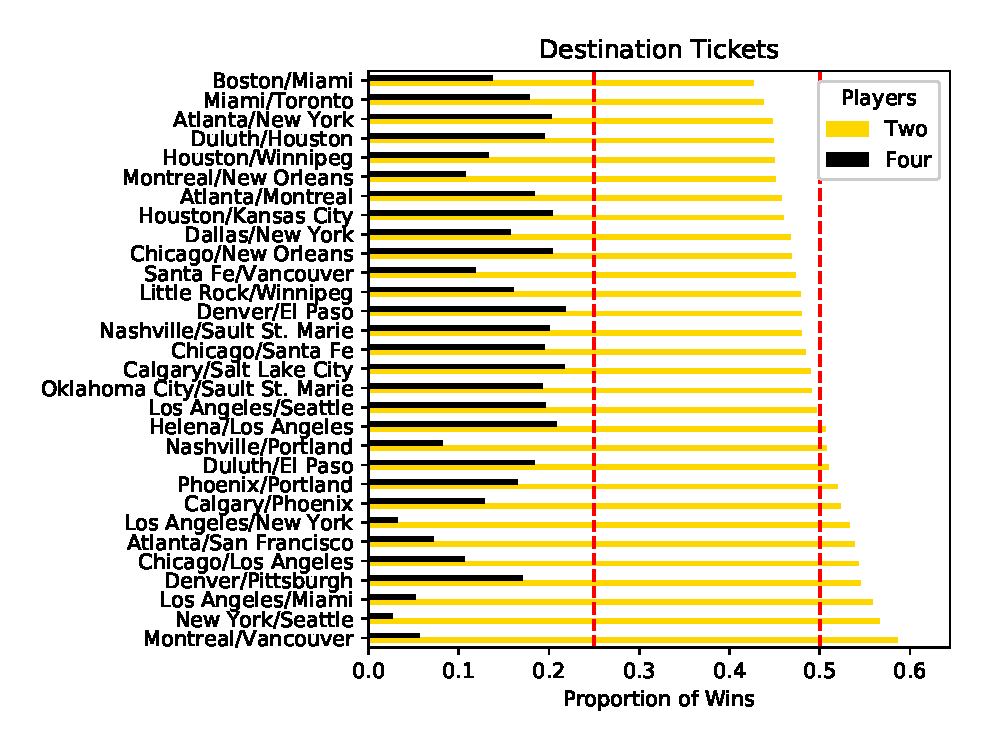
\includegraphics[scale=.65]{figures/destination_tickets}
\caption{For each Destination Ticket,
the proportion of two-player and four-player games that 
the player with the Destination Ticket won.
The vertical red lines at $1/4$ and $1/2$ represent
the expected proportion of games players would win
if Destination Tickets had no effect.}
\label{fig:tickets}
\end{figure}
\begin{multicols}{2}

The vertical red lines at .25 and .5 indicate
the expected proportion of wins if Destination Tickets
had no effect on winning: players in two-player games
would win half the time and players in four-player games
would win a quarter of the time.

In two-player games, there are 13 Destination Tickets 
that win more than the expected $50\%$ of games.
In four-player games, there are only eight Destination Tickets
that clearly win more than the expected $25\%$ of games plus
another four on the borderline.
That is, out of the 30 Destination Tickets, roughly a third
in both two- and four-player games win more than expected.
The implication is that a randomly chosen Destination 
Ticket is not advantageous.
However, a subset of Destination Tickets--approximately the same
set for both two- and four-player games--wins more often than expected.
The ones that win the most from the subset are Montreal to Vancouver,
New York to Seattle, and Chicago to Los Angeles.
An inspection of \cref{fig:board} shows that the paths between 
these three Destination Tickets are some of the longest on the board 
and also have some of the longest routes.

In the rest of this section, we investigate the characteristics of
Destination Tickets that most closely correlate with
winning.
We begin in the next subsection by developing a measure
of the difficulty of connecting one city to another.

\subsection{Effective Resistance}
The \textit{Ticket to Ride} board can mathematically
be interpreted as a graph where cities represent
nodes and routes represent edges.
Therefore to analyze the difficulty of connecting a
pair of cities we can frame the problem in graph theoretic language.
One of the most powerful and natural measures
between two nodes on a graph is effective resistance
\cite{ellens2011effective}.
Imagine that the \textit{Ticket to Ride} board was
a large electrical circuit with a unit current
entering at city $a$ and leaving at city $b$.
Effective resistance is a measure
of how much work a current needs to exert
to get from $a$ to $b$.
In general, the number of paths and length of routes 
determine the effective resistance:
two cities with fewer paths and longer routes
have a higher effective resistance between them
than two cities with many paths and shorter routes.
We calculate the effective resistance for each 
Destination Ticket in order to gain insight
into what makes players with some Destination Tickets
win more often than players with other Destination Tickets.

On a small graph, effective resistance can be calculated
by repeatedly applying the following rules.
Consider two edges with resistances $r_1$ and $r_0$.
If the two edges are in series (edge 1 connects node $i$ to $j$
and edge 2 connects node $j$ to $k$), then the resistance between
$i$ and $i$ is $r_1 + r_2$.
If the two edges are in parallel (both edge 1 and edge 2 connect
node $i$ to $j$), then the resistance between $i$ and $j$
is $(1/r_1 + 1/r_2)^{-1}$.

On a large graph like the \textit{Ticket to Ride} board, 
we need a more robust strategy.
We use two separate algorithms to find the effective resistance
of Destination Tickets
\cite{ellens2011effective, wu2004theory}.
Both algorithms calculate the effective resistance by finding 
the eigenvalues of the Laplacian matrix for a given graph.
The Laplacian is the degree matrix $D$ minus the adjacency
matrix $A$ where $D_{i,i}$ is the weighted degree of node $i$
and $A_{i,j}$ is the resistance of the edges between nodes
$i$ and $j$.

We let the weight between two cities be the number
of trains of the route connecting them.
In the case that there are two routes between cities,
we let the weight be $(1/r + 1/r)^{-1}=r/2$ where
$r$ is the number of trains of each route.

In the next subsection, we calculate the effective
resistance of all Destination Tickets as a tool
to find what most closely correlates with winning.

\subsection{Winning \& Effective Resistance}

In \cref{fig:resistance},
Destination Tickets are plotted by their effective resistance
and minimum path length.
Recall that the reward for connecting a Destination Ticket
is the length of the shortest path between its two cities.
Since effective resistance measures the difficulty of
connecting the two cities, the line of best fit in \cref{fig:resistance}
indicates reward per difficulty.
The Destination Tickets above the line of best fit have
a higher reward per difficulty whereas those below the line of best fit
have a lower reward per difficulty.

Our results appear in \cref{fig:correlation_table}
and \cref{fig:resistance}.

\end{multicols}
\begin{figure}
    \centering
    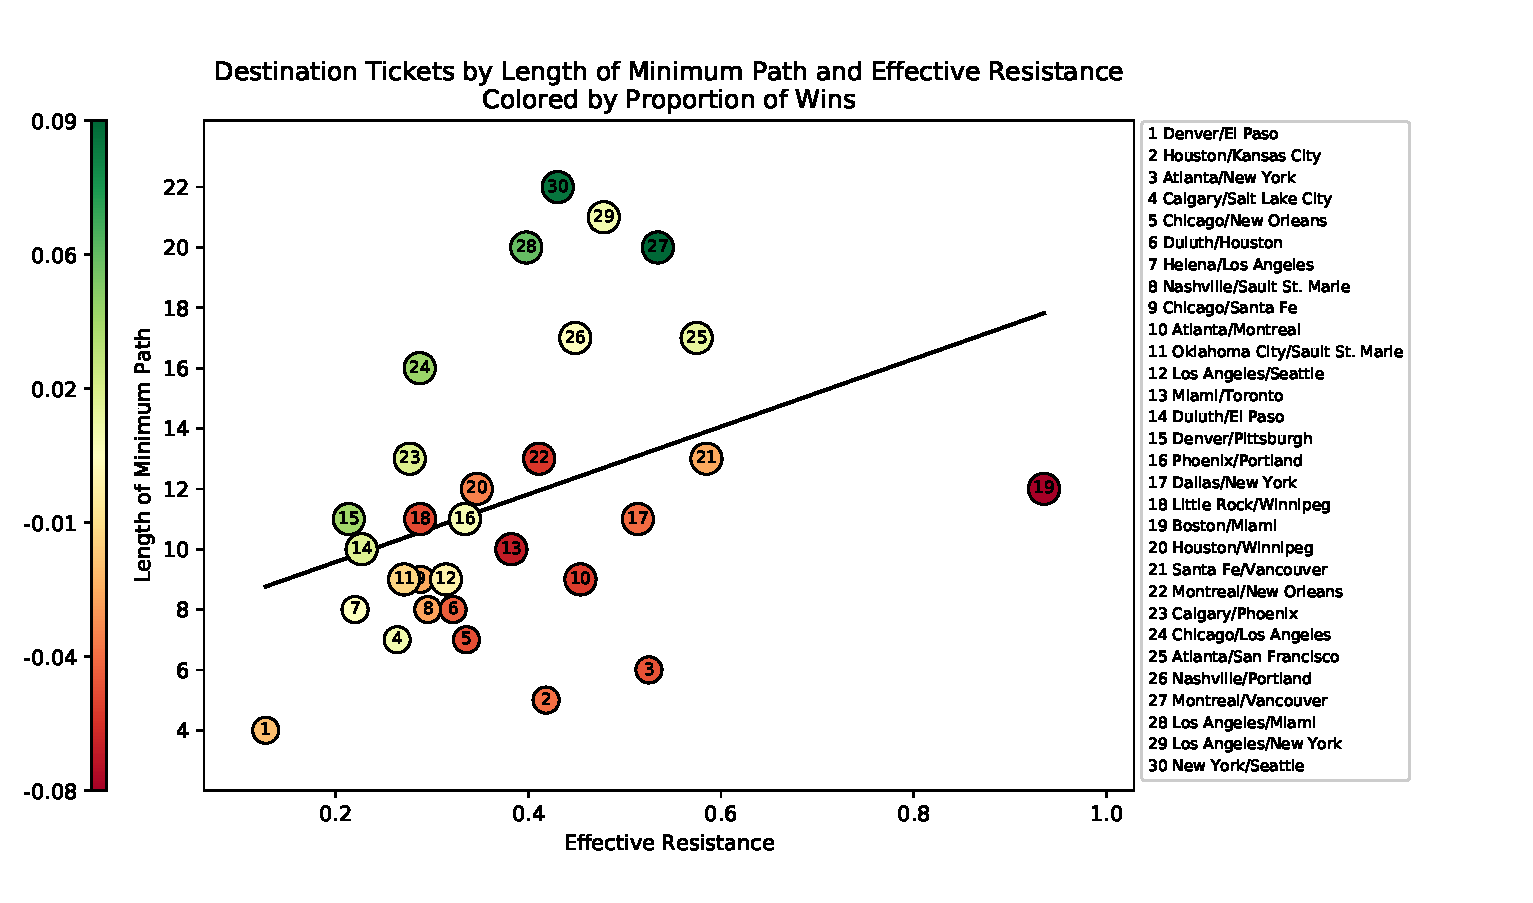
\includegraphics[scale=.5]{figures/resistance_aggregate}
    \caption{Destination Tickets plotted by their effective
    resistance and minimum path length and colored
    by overall proportion of wins.
    The line of best fit gives an approximation of the
    Destination Tickets that have a higher reward per difficulty
    (above the line).
    Note: the $9^{th}$ Destination Ticket 
    is obscured by the $11^{th}$.}
    \label{fig:resistance}
\end{figure}
\begin{multicols}{2}

\begin{figure}[H]
    \centering
    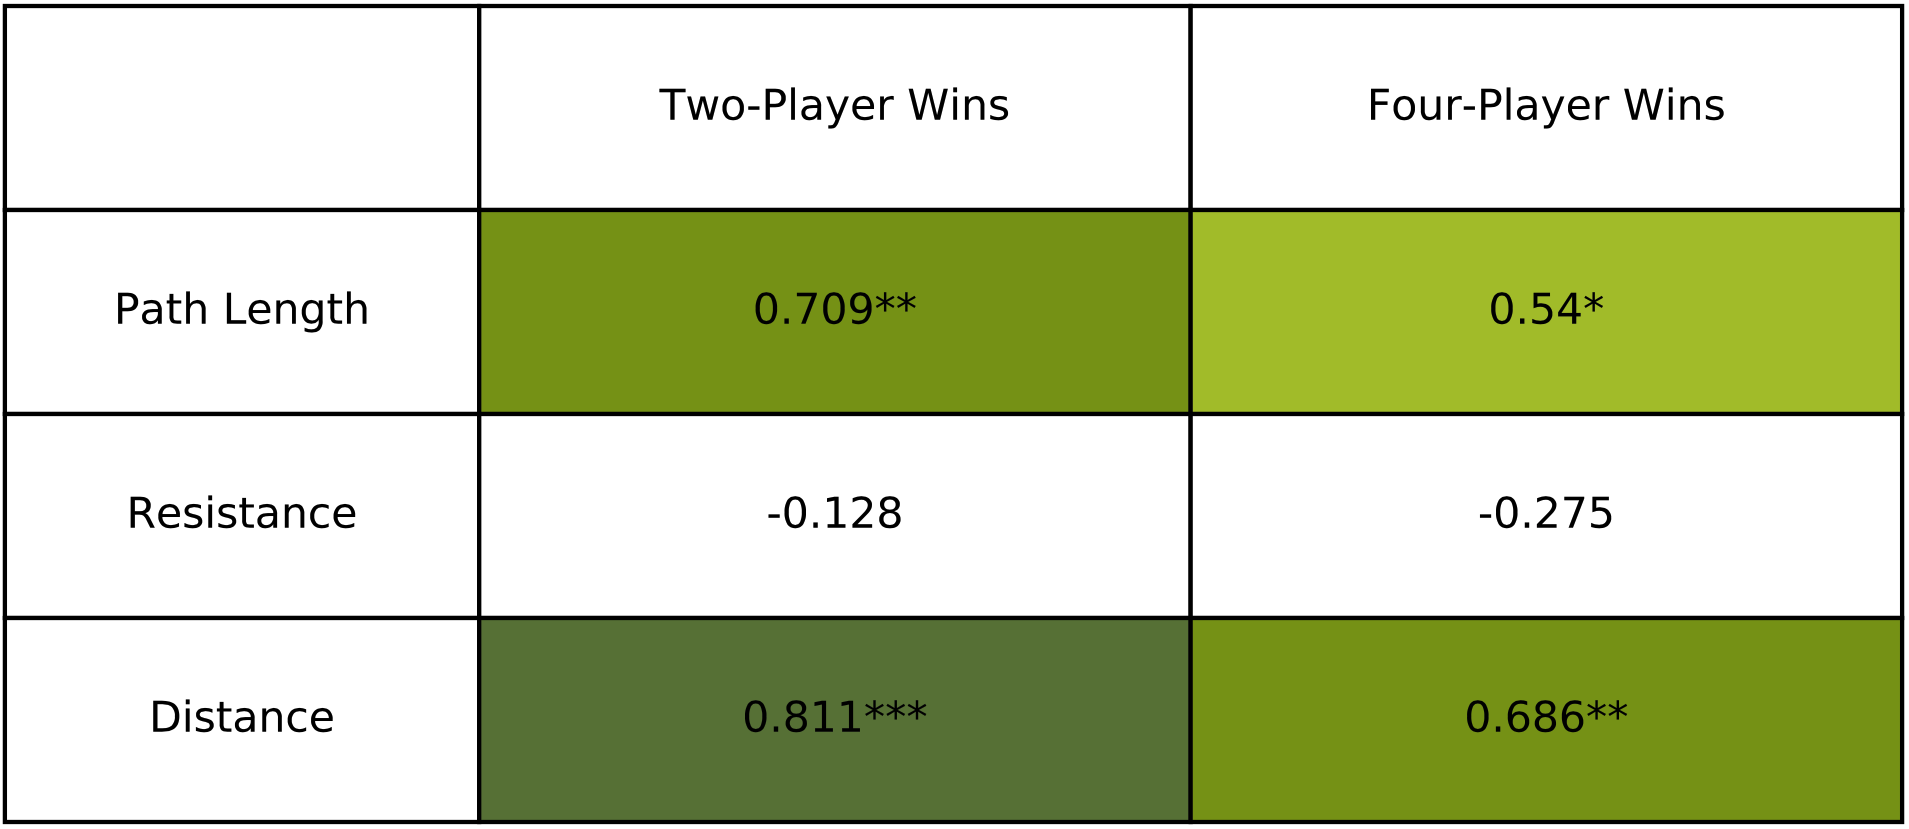
\includegraphics[scale=.12]{figures/pearsons_table.png}
    \caption{The Pearson correlation statistic between
    the win proportion of Destination Tickets
    and measures of difficulty.
    A single asterisk (in light green) indicates a p-value
    below 1E-2. Double asterisks (in green) indicate a
    p-value below 1E-4. Triple asterisks (in dark green)
    indicate a p-value below 1E-6.}
    \label{fig:correlation_table}
\end{figure}
